\begin{figure}[t]
  \begin{tikzpicture}[scale=0.75,transform shape]
  \SetVertexMath
  \GraphInit[vstyle=Simple]
  \SetGraphUnit{2.5}
  \Vertex[x=0,y=2,L=$S$,NoLabel=false,LabelOut=true,Lpos=180]{A}
  \Vertex[x=1,y=0]{B}
  \Vertex[x=2,y=1.5]{C}
  \Vertex[x=2.5,y=4.2]{D}
  \Vertex[x=4,y=3.5]{E}
  \Vertex[x=4.5,y=2]{F}
  \Vertex[x=5.5,y=4]{G}
  \Vertex[x=7,y=3]{H}
  \Edge[label=$5$](A)(D)
  \Edge[label=$4$](A)(B)
  \Edge[label=$4$](D)(C)
  \Edge[label=$5$](F)(H)
  \Edge[local,label=$3$,color=blue](A)(C)
  \Edge[local,label=$3$,color=blue](C)(B)
  \Edge[local,label=$2$,color=blue](D)(E)
  \Edge[local,label=$3$,color=blue](C)(E)
  \Edge[local,label=$1$,color=blue](E)(F)
  \Edge[local,label=$2$,color=blue](E)(G)
  \Edge[local,label=$3$,color=blue](G)(H)
\end{tikzpicture}
\centering
\caption{The output of Prim's algorithm given the example classroom graph from
\Fref{fig:class-graph} as input. Blue edges represent edges in the output
spanning tree. The initial vertex $S$ was chosen arbitrarily. It is not
difficult to see that the output spanning tree would be the same had the
algorithm selected any other initial vertex.}
\label{fig:class-graph-mst}
\end{figure}
